%\pgfdeclarelayer{background}
%\pgfdeclarelayer{foreground}
%\pgfsetlayers{background,main,foreground}

\pgfplotsset{
	axis background/.style={fill=none},
	%tick style=mygrey2,
	%tick label style=mygrey2,
	grid=none,
	%xtick pos=left,
	%ytick pos=left,
	tick style={
		major grid style={style=white,line width=1pt},minor grid style=white,
%		major grid style={style=white,line width=1pt},minor grid style=mygrey3,
		%tick align=outside,
	},
	%minor tick num=4,
}

\begin{figure}[tb]
	\centering
	 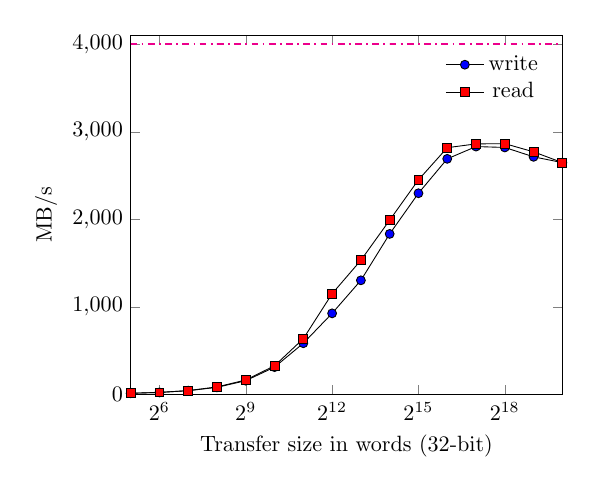
\begin{tikzpicture}[scale = 0.8]
	 \begin{axis}[
	 xmode=log,
	 log basis x={2},
	 xlabel=Transfer size in words (32-bit),
	 ymin=0,
	 ymax=4100,
	 %ymin=200,
	 %ymax=400,
	 xmax = 1048576,
	 xmin = 32,
	 ylabel=MB/s,
%	 legend style={at={(0.3,0.8)},anchor=north}
	 legend pos=north east,
	 legend style={draw=none}
	 ]    

	\addplot [mark=*,mark options={fill=blue}] plot coordinates {
		(32,     11.1)
		(64,     20.3)
		(128,    41.0)
		(256,    78.8)
		(512,    155.0)
		(1024,   310.0)
		(2048,   583.0)
		(4096,   924.6)
		(8192,   1302.1)
		(16384,  1832.8)
		(32768,  2297.8)
		(65536,  2691.1)
		(131072, 2831.3)
		(262144, 2821.2)
		(524288, 2713.9)
		(1048576,2647.7)	
	}; 
	 \addplot [mark=square*,mark options={fill=red}] plot coordinates {
	 	(32,     11.1)
	 	(64,     21.0)
	 	(128,    41.4)
	 	(256,    83.5)
	 	(512,    162.8)
	 	(1024,   325.5)
	 	(2048,   635.2)
	 	(4096,   1148.9)
	 	(8192,   1531.9)
	 	(16384,  1990.4)
	 	(32768,  2451.0)
	 	(65536,  2818.5)
	 	(131072, 2862.0)
	 	(262144, 2864.5)
	 	(524288, 2771.1)
	 	(1048576,2647.7)
	 }; 
	 
	 \addplot [color=magenta,thick,dash dot] plot coordinates {
	 	(32,     4000)
	 	(64,     4000)
	 	(128,     4000)
	 	(256,     4000)
	 	(512,     4000)
	 	(1024,     4000)
	 	(2048,     4000)
	 	(4096,     4000)
	 	(8192,     4000)
	 	(16384,    4000)
	 	(32768,    4000)
	 	(65536,    4000)
	 	(131072,   4000)
	 	(262144,   4000)
	 	(524288,   4000)
	 	(1048576,  4000)	
	 };

	 \legend{write\\read\\}
	 \end{axis}
	 \end{tikzpicture}	
	
	\caption[]{RIFFA loopback throughput.} 
	\label{riffa_loopback_bw}
	
\end{figure}
